%------------------------------------------------------------------------
% Chapter:  Differential evolution
%------------------------------------------------------------------------

\chapter{Differential Evolutionary Algorithm \label{diff}}
\section{Refinement via evolutionary algorithms \label{diff-evol}}

Every time we measure some physical effect and wish to understand
how this effect works, we want to determine the parameters of a 
model function that will replicate the observations. The term 
refinement refers to the process by which the parameters of the
function are tuned such as to give the best agreement between
the observed and calculated values. The term {\it best agreement}
merits careful definition, for right now it is sufficient to say
that the sum over all squared differences between the observations and the 
calculations shall be minimized. Thus, refinement is but a special
case of general optimization. A very different example for an 
optimization could be the task to place as many integrated 
circuits into a chip and simultaneously achieve the fastest computations.
Quite well known is the traveling salesman problem. Here the 
optimization task requires to find the shortest route that 
visits a number of spots distributed in space.  

By far the fastest refinement technique is a least squares algorithm.
Such an algorithm can always be applied if we can describe the 
physical effect as a function of parameters:
\begin{equation}
  y ~=~ F(p_{0}, p_{1}, ..., p_{n}),
\end{equation}
and all the partial derivatives $\partial y/ \partial p_{i}$ can 
be calculated, either analytically or numerically. For each 
observed value y$_{obs}$, we calculate a value y$_{calc}$ and 
minimize the value of a weighted residual wR:
\begin{equation}
   wR = \sqrt{\frac{\sum_{i} w_{i} (y_{obs}(i) - y_{calc}(i))^2}
                   {\sum_{i} w_{i} y_{obs}(i)^2}}
\end{equation}
Here each difference is multiplied by a weight w$_{i}$ that reflects
the uncertainties of the experimental values. In case of crystal 
structure analysis, the observed values would be the observed 
intensities in a diffraction pattern and the calculated values 
those intensities that were calculated based on a structural model. 
Model parameters will be the lattice parameters, the positions
of the atoms in the unit cell, atomic displacement parameters etc.
as well as experimental parameters, such as the background.
Under the assumption that we have a periodic crystal, the 
partial derivatives of the intensity with respect to lattice
parameters, atom positions etc., can all be derived analytically.

For disordered structures, the situation becomes more complicated.
Except for a few special cases like stacking faults or short-range
order problems, no general analytical function straightforwardly 
links the disorder parameter to the intensity. The intensity 
can still be calculated from structural models. The simulation,
however, usually involves the application of random choices 
to generate part or all of the atom positions, and the analytical
derivative of the intensity with respect to the order parameter
is no longer available. A numeric calculation of the derivatives
involves the repeated simulation of a new model for each parameter
and is very time consuming.

Other, general optimization problems also do not have an 
analytical derivative. For the traveling salesman problem, for 
example, no derivative exists between the sequence in which the 
spots are visited and the resulting length of the trip.

Under these circumstances, optimization algorithms are required 
that can find the best solution without calculation of the 
partial derivatives. Evolutionary algorithms are such an alternative to 
least squares refinement algorithms.

These algorithms loosely mimic the evolution of plants and animals
under an environmental pressure. In contrast to a least squares
algorithm they usually do not operate with a single parameter set
but a group of parameter sets.

\begin{figure}[htbp]
   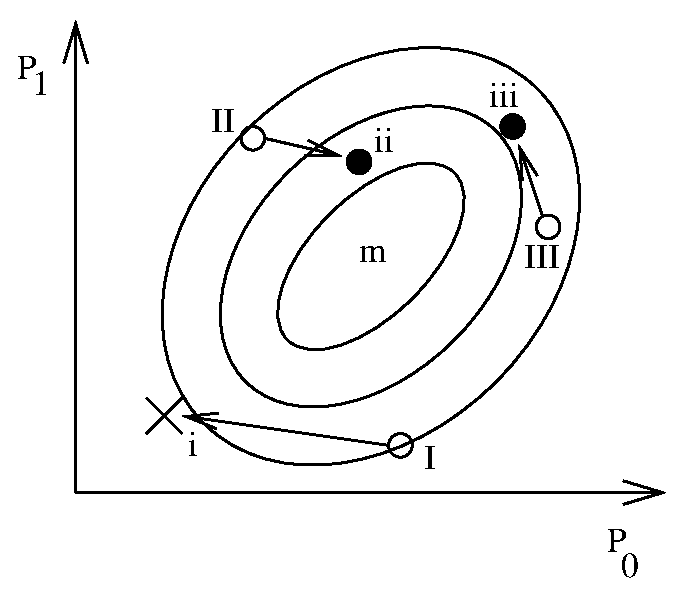
\includegraphics[angle=0,scale=0.65]{refine.evol.eps}
   \caption{Schematic sketch of an evolutionary algorithm.
    Two parameters P$_{0}$ and P$_{1}$ are refined in the search
    for the optimum solution. The ellipsoidal lines represent 
    lines of equal R-values. The global minimum is at point m.
    Members I, II, and III generate the new members i, ii, and iii
    by modification of the original parameter values.
    The new members ii and iii have an improved R-value, while
    member i has a worse R-value compared to the original member I.}
   \label{evo-evol}
\end{figure}

The algorithm begins by creating a group of parameter sets, see Fig.
\ref{evo-evol}. Each group 
member is a list of parameter values M:[$p_{0}, p_{1}, ..., p_{n}$],
and for each member the R-value is calculated. Next, a new group of
parameter sets is generated. Several different algorithms for this
step exist. One possibility is to change each parameter by a Gaussian
distributed random number with mean zero, which is added to the original
parameter value. The variance of this distribution will vary from
parameter to parameter. The lattice constants, for example will
need another variance than the angles. In Fig. \ref{evo-evol}
the members I, II, and III create in turn the new members i, ii, and iii.
This modification  of a single parent member is comparable to the 
genetic mutation in biological systems. Most systems apply a second
modification, that mixes the parameter values of two different parent
members, a process that roughly resembles the sexual replication.

Once the new group of members has been generated, their R-values are 
calculated in turn. In the example child members ii, and iii have a
smaller R-value compared to their respective parent members, while
child i has a higher R-value than its parent. The next task to decide 
which members of the old parents and children shall be retained and 
form the next parent group from which the next children group is to be
generated. A number of different approaches exist for this task. One
option is to compare a child with its immediate parent and to keep the 
better of these two. In the situation depicted in Fig. \ref{evo-evol},
this would choose the parameter sets I, ii, and iii as parents for the
next generation. Another approach is to combine all parents and all
children into one group. From this group the N best are chosen as 
parents for the next generation. In Fig. \ref{evo-evol} this would
give the parameter sets ii, III, and iii as parents for the next 
generation, since these three sets have the three lowest R-values.

As the parameter values change from generation to generations, those
members survive that have better R-values. As consequence, the parameter
value evolve towards the minimum R-value. If the landscape of R-values
is more rugged compared to the simple situation of 
Fig. \ref{evo-evol}, one has to be careful not to refine into a
local minimum instead of the global minimum. The literature on 
evolutionary algorithms extensively deals with this issue.
%------------------------------------------------------------------------

\section{The differential evolutionary algorithm \label{diff-price}}

The essential feature of the differential evolutionary algorithm, 
introduced by Price and Storn \cite{prstla2005}, is the process, by which
new children are generated.

\begin{figure}[htbp]
   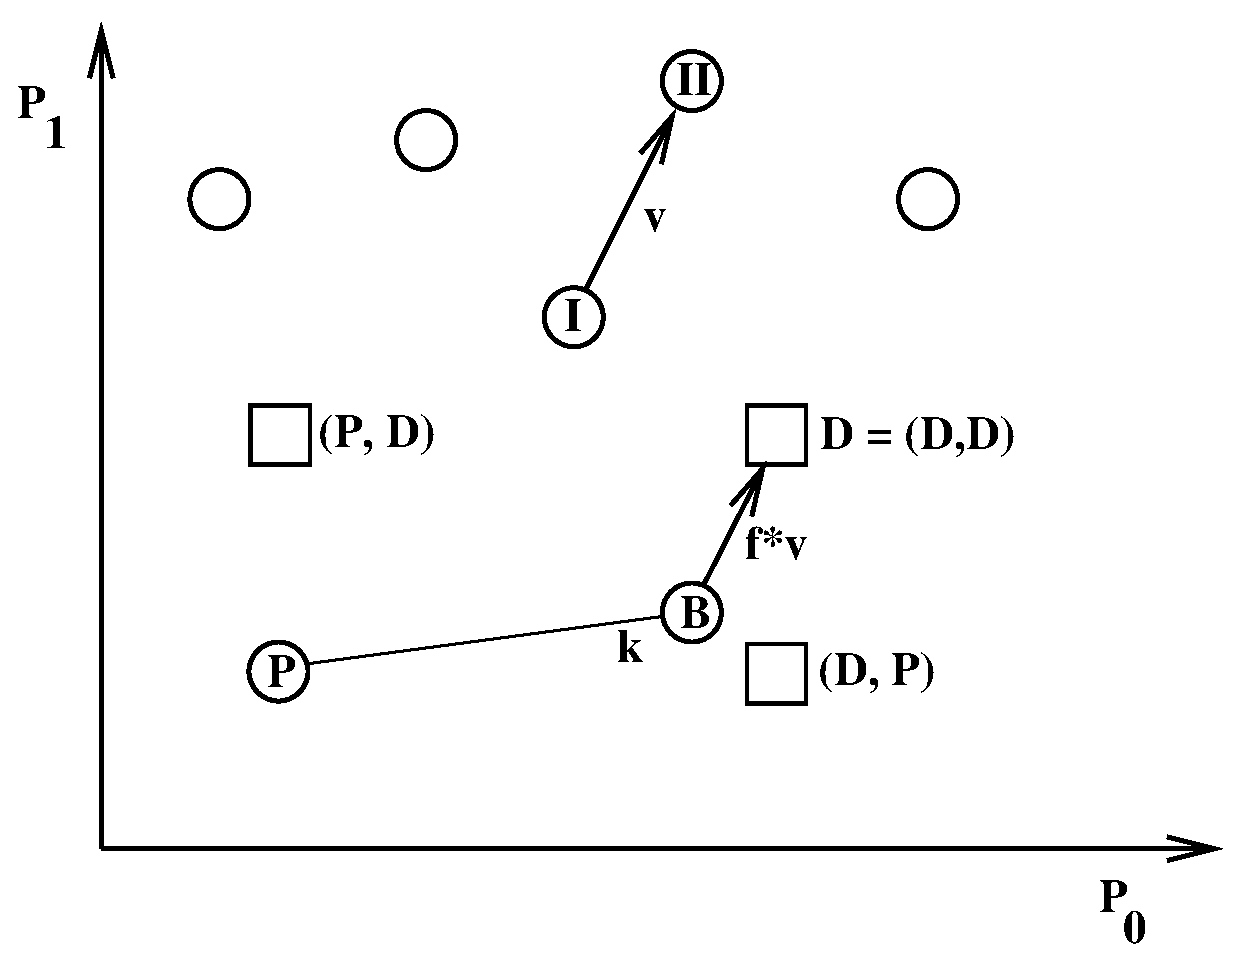
\includegraphics[angle=0,scale=0.45]{refine.diffev.eps}
   \caption{Schematic diagram of the differential evolution algorithm.}
   \label{evo-select}
\end{figure}

The algorithm picks in random sequence all members of the current 
generation, shown as circles in Fig. \ref{evo-select}. The current
parent has been marked by P in the figure. Another member, the base B 
is chosen at random. Next, two other members are also 
chosen at random, members I and II in Fig. \ref{evo-select}. The
differential evolutionary algorithm then calculates the difference vector
$\vec{v} ~=~ \vec{II} - \vec{I}$ between these two parents. This difference
is the part of the algorithm that coined the name. The difference vector
is multiplied by a factor f and added to the base member. 
All four members are different members of the population. The
scale factor f is a variable that is used to control the refinement
properties of the differential evolutionary algorithm. In general it
should be somewhat smaller than one. The sum of the base member and the
difference vector is a general point in parameter space, called the 
donor D. The donor D is the basic modification of th original parent
vector. In contrast to other evolutionary algorithms, there is no
direct connection between the parameter values of the parent P and its
modification, the donor D. 

After the determination of the donor D, the differential evolutionary
algorithm allows for a mixing of the parameter values between the 
parent P and the donor D. By random choice, parameter values are taken
either from the donor or from the parent. To ensure that the parent 
is not replicated, one parameter value is always taken from the 
donor D. The probability, by which the other parameters are taken from 
the donor D is called the cross over probability. Fig. 
\ref{evo-select} also illustrates the cross over process. If 
both parameters happen to be taken from the donor, the final child is the
donor itself. If parameter $p_{0}$ is taken from the donor and 
parameter $p_{1}$ taken from the parent, the child will be the position
labeled (D,P). Alternatively, if parameter $p_{0}$ is taken from the 
parent and parameter $p_{1}$ from the donor, the child will be the
position labeled (P,D). Thus the cross over leads to a mixing of 
the parameter values of the donor D and the parent P. It depends on the
refinement problem at hand, whether the cross over probability should 
favor parameters of the donor or the parent in order to ensure convergence. 

Once children have been created for all parents, their R-values are 
computed. The differential evolutionary algorithm compares the 
R-values of each parent and its immediate child. Whoever has the 
lower R-value survives and is treated as parent for the next generation.

Several modifications to this basic differential evolutionary
algorithm exist. The first modification concerns the choice of the
donor base B. In the standard algorithm, the donor base is chosen
randomly among the members of the population. As an alternative one
can decide to take the current best member as donor base for all
children. This will search predominantly in the neighborhood of the
current best member and thus speed up the convergence into the 
minimum close to the current best member. If, however, this minimum
is a local instead of the global minimum, chances are higher that 
all children will be within this local minimum as well.

Another alternative allows to add the scaled difference vector to
any point along a straight line between parent and donor base, the 
line marked k in Fig. \ref{evo-select}. A control variable 
{\em k} chooses the point. I the usual definition, the donor base 
is chosen if k=1 and the parent if k=0, and any point in between
for intermediate values of k. In principle k is not limited to 
the interval [0:1], and \Diffev does not limit your choice. 

Choosing the surviving members allows for another modification of the
original algorithm. Instead of a pairwise comparison of parent and
child, one can also group all M parents and all N children into one group.
Those M member of this combined group that have the lowest R-values
survive and are used as parents for the next generation. The status of
original parent or child is not taken into account. This approach will
usually lead to a faster convergence, albeit at the risk of convergence 
into a local minimum. If the number of children is increased 
beyond the number of parents, the 
{\em evolutionary pressure} increases and the convergence is generally
enhanced.

%------------------------------------------------------------------------

\section{Termination criteria \label{diff-term}}

Several different criteria may be used to terminate an evolutionary
refinement. 

\begin{itemize}
  \item {\bf Global minimum has been reached}\\
     If the values that correspond to the global minimum is
     known, the refinement can stop, once the lowest trial value falls
     within a defined threshold above this value. Unfortunately, in 
     case of structure refinements, the lowest R-value cannot be known
     before hand and this criterion is not well suited.
  \item {\bf Predefined number of refinement cycles}\\
     If the best R-value does not decrease for a given number of 
     generations, chances are that we are very close to the global minimum.
     Unfortunately, one can never know whether the refinement may not
     improve after just a another few generations. This criterion may, however,
     be used to determine a good refinement strategy. The main variables
     to the differential evolutionary algorithm are the population size, 
     the scale factor f by which the difference vector is multiplied, 
     and the cross over probability. If refinements with different 
     settings for these control parameters are allowed to run for a 
     given number of generations. Those control parameters that lead to
     the lowest R-values after these generations can then be taken as 
     good parameters for further refinement problems.
  \item {\bf Population statistics}\\
     For diffraction data, it is straightforward to calculate an expected
     R-value. The refinement can be stopped, once the best R-value 
     reaches this value, or at least comes close. Another choice could
     be to wait until all R-values have dropped to within a defined 
     range of R-values above the expected R-value. The corresponding
     parameter range may then be inspected to determine the corresponding 
     parameter uncertainties. If the model is insufficient, one may never
     reach this situation. Instead one could terminate the refinement
     once all R-values have become very similar to each other. If the
     lowest R-value is significantly above the R-expected one should 
     run the refinement again with different starting parameters, of 
     different control parameter settings to exclude convergence into a
     local minimum. If the parameters refine into the same minimum, the
     model should be analyzed and hopefully be improved.
  \item {\bf User intervention}
     The last choice is to run the refinement indefinitely and to 
     terminate the refinement manually be the user. Given the many 
     different disorder problems that \Diffev may face, this is the main
     termination criterion offered at present.

\end{itemize}

\section{Optimizing the performance \label{diff-opti}}

The examples in this section use the example from chapter
\ref{example}. Details given here are sketchy, refer to chapter
\ref{example} for full details.

Choosing the best setup for the refinement is in itself an abstract 
optimization task. One should choose those values for the control
parameters that will cause the refinement to find the global minimum
with the least amount of function calls. With regards to the
differential evolutionary algorithm one needs to select the best 
values for:

\begin{itemize}
  \item {\bf Population size}
  \item {\bf Scale factor f}
  \item {\bf Cross over probability}
  \item {\bf Choice of donor base}
  \item {\bf Selection mode} 
  \item {\bf Local search probability}
\end{itemize}

The actual values that give the best performance will depend on the
refinement problem at hand. See the discussion in chapters 2 and 
3 of \cite{prstla2005} for a further details. In the following we
show a few examples that illustrate how to find good parameter 
settings.

\subsection{Population size}

\begin{figure}[htbp]
   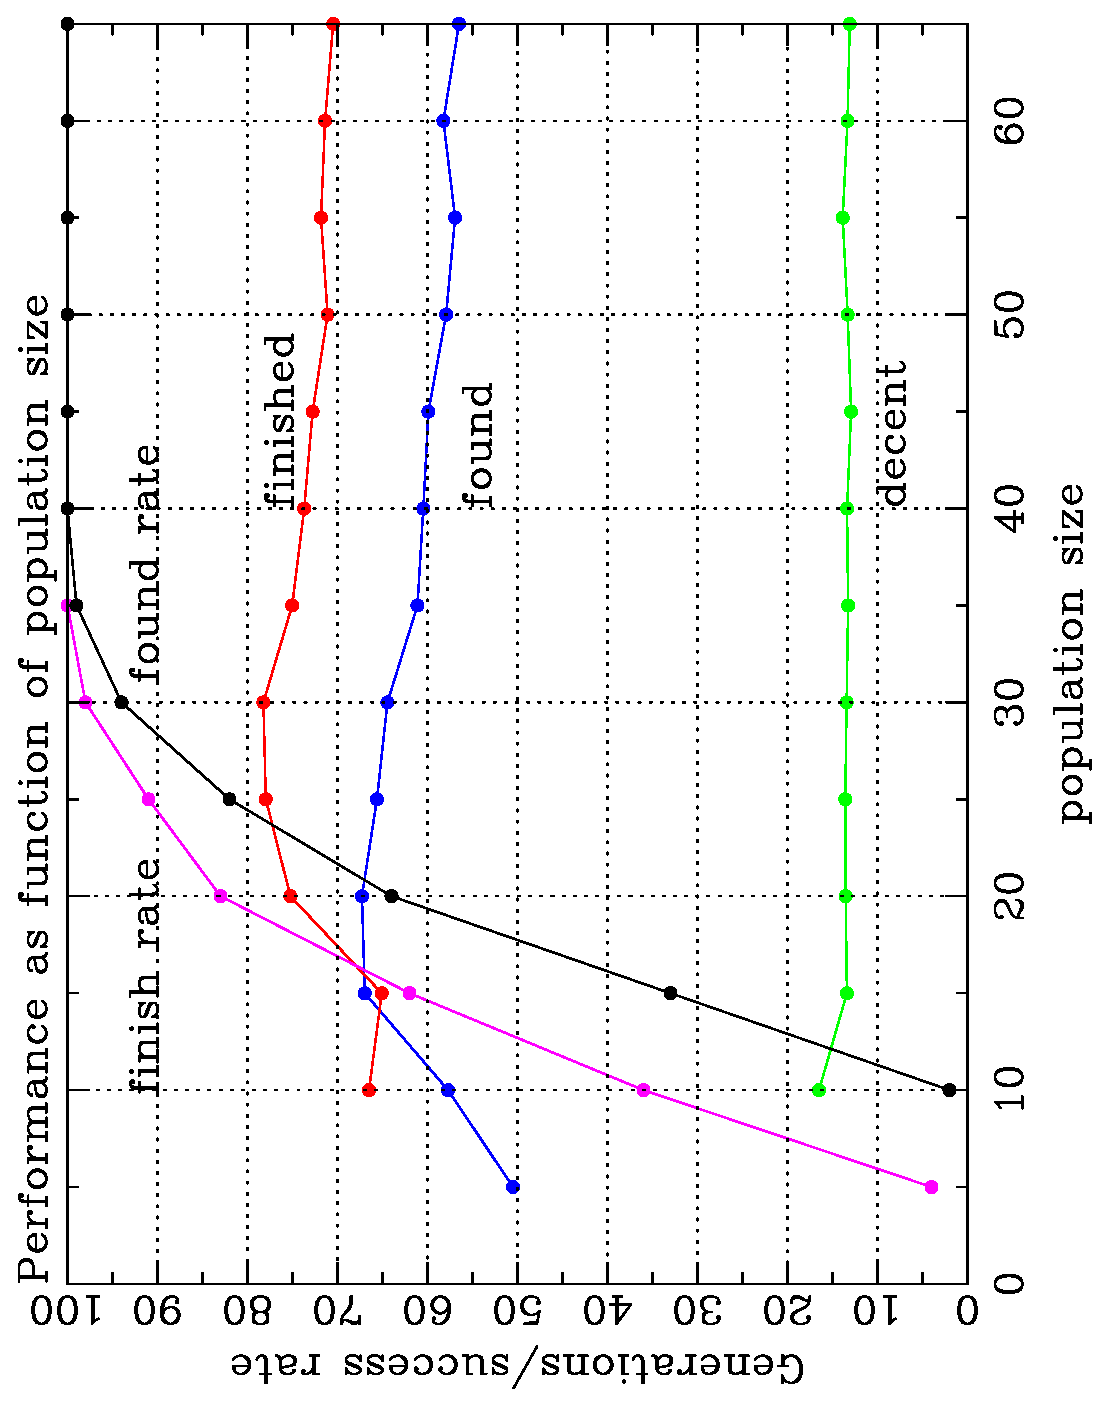
\includegraphics[angle=270,scale=0.45]{refine.pop.eps}
   \caption{Success rate as function of population size.}
   \label{evo-pop}
\end{figure}

If the population size is small, few permutations exist between the 
members of the population and there will be few locations that are
searched in the parameter space.

Fig. \ref{evo-pop} shows the effect the population size has on the
refinement of the modified arctan function. This function requires 
three parameters, and parameters 2 and 3 pose a challenge due to the 
high noise present in the data. The true parameters for the example
function were $P_{1}=100;~P_{2}=100.23;~P_{3}=0.1$. The refinement was run
for population sizes from 5 to 65 members. The donor base was chosen
at random, and the selection mode took the best members from 
the combined group of parents and children. The local search mode was 
switched off. The refinement was
considered successful, if the R-value fell below a given threshold. 
Due to the special function, this meant that the parameters are close
to the true parameters and that the refinement will from here on 
converge into the global minimum. The refinement was allowed to run
for 100 generations. Refinements that did not reach the global minimum
or did not finish to refine to the global minimum were considered 
failures. At each population size, the refinement
was repeated 100 times. Fig. \ref{evo-pop} shows the performance as
function of population size. The blue and red curves show the number 
of generations required to get close to the global minimum, respectively 
to finish refining into the global minimum. The black and purple curves
show the percentage of refinements that came close to the minimum, 
respectively finished refining into the global minimum within the 
allowed 100 generations. 

A population size of about 40 members is needed to ensure 
a 100\% success rate. At smaller population sizes, a larger fraction of
the refinements does not find the minimum and thus the refinement 
cannot be considered satisfactory. If the population size is increased
beyond 40, the number of generations required to get close to the 
minimum, respectively to finish refining into the global minimum 
decreases slightly. The increase in function calls due to the population
size increase is, however, higher than the gain obtained by faster 
refinements.

\subsection{Scale factor and cross over probability}

To test good values for these two parameters, the population size of 
40 was adapted according to the observations on the population size.
Both factors were chosen randomly in the interval [0:1]. As in the
previous investigation, the refinement was considered successful, if
the parameters reached the true values within 100 generations.

\begin{figure}[htbp]
   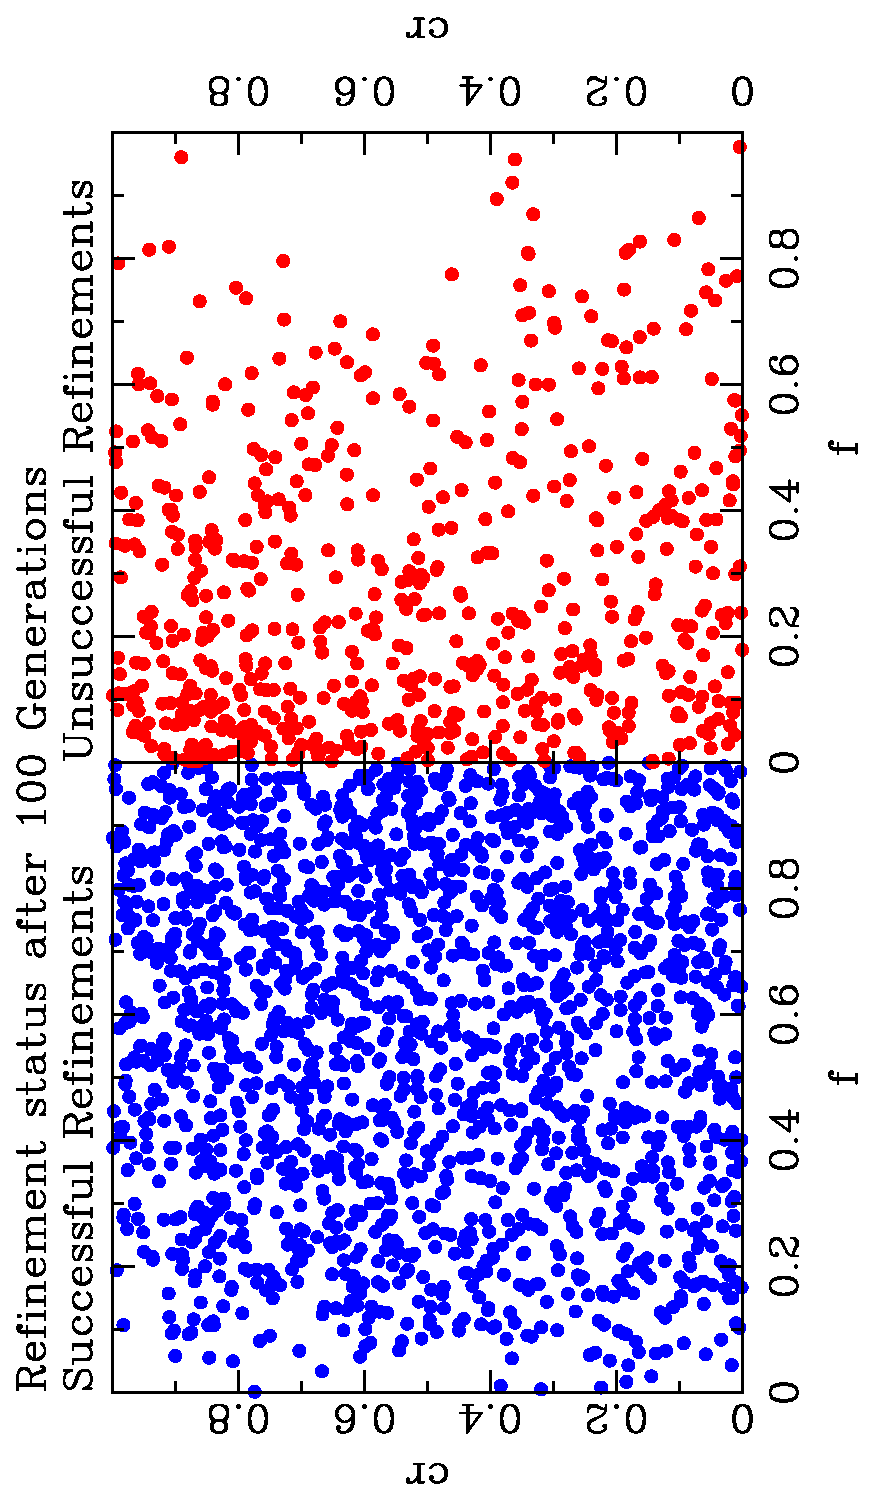
\includegraphics[angle=270,scale=0.55]{refine.fcr.eps}
   \caption{Success rate as function of scale factor f and
    cross over probability cr.}
   \label{evo-fcr}
\end{figure}

The figure shows that successful refinements of this example function
require a scale factor
that should be closer to 1. For very small scale factors, the 
algorithm effectively searches in the local environment of the 
donor base instead of a wide parameter range. In this example, this
increases the chance of refining into a local minimum.

\subsection{Local search probability}

A cut through R-value space along $P_{3}$ at $P_{1}$ and $P_{2}$ at their
respective optimum values shows a narrow minimum around the optimum
value of 0.1. This behavior might indicate that a local search around the
members might enhance the convergence into this narrow minimum. To
test this, two different test were performed, in which the local search 
probability was systematically varied from 0 to 1. 

For both tests with different local search options, otherwise identical 
control variables were used. The population size was set to 40 members,
the scale factor was 0.81 and the cross over probability 0.8. The donor
base was chosen randomly and the best members of the combined parent/children
group were selected. For each local search probability the refinement
was repeated 100 times.

Figure \ref{evo-lo} shows the number of generations required to 
find a parameter combination close to the global minimum (blue), the total
number of generations required to refine very close to the global minimum
(red), the number of generations required from the time the first 
parameter set is close to the global minimum until the global minimum is
reached (green), the percentage of refinements that came close to the 
minimum (black, and the percentage of refinements that finished refining
into the global minimum (purple).

\begin{figure}[htbp]
   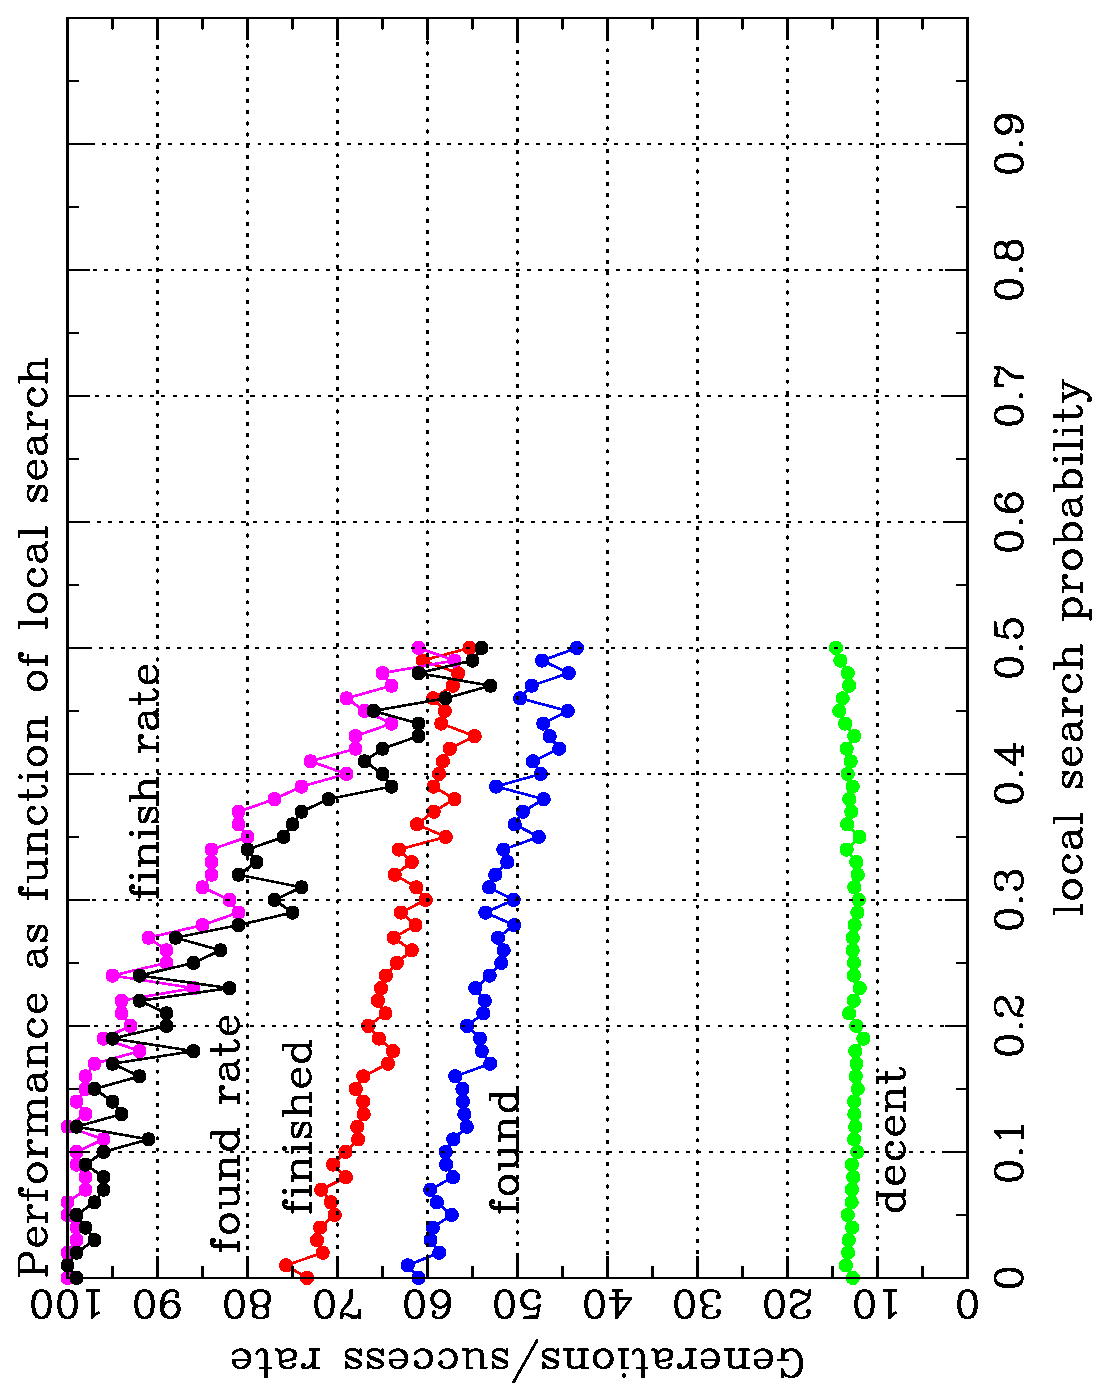
\includegraphics[angle=270,scale=0.34]{refine.lo.ada.eps}
   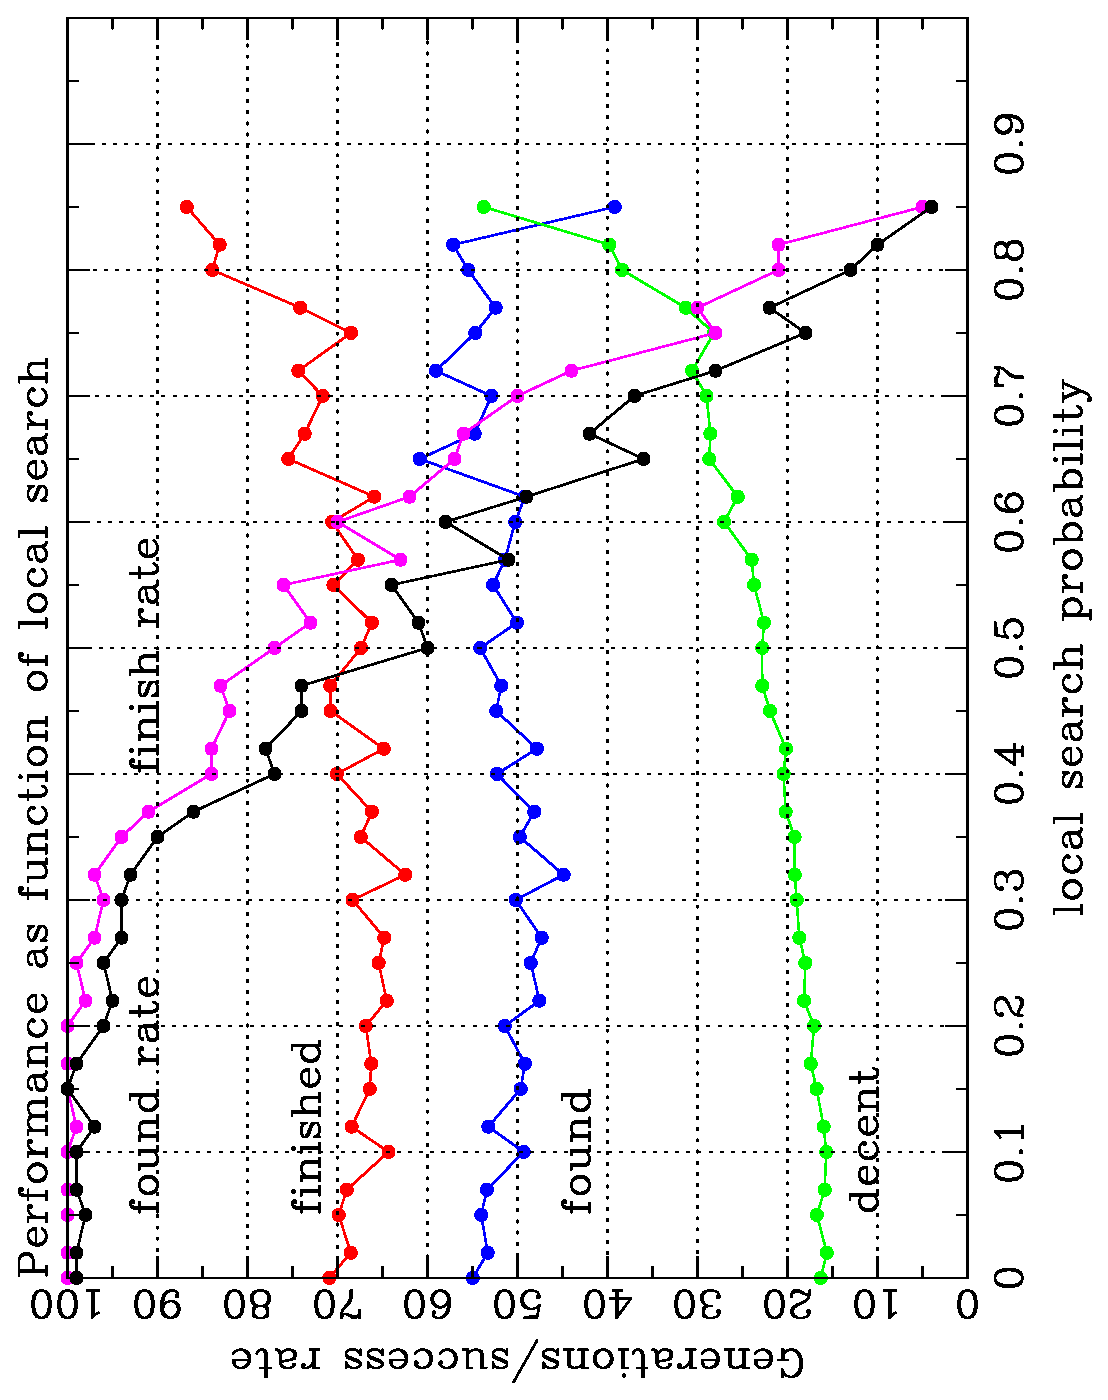
\includegraphics[angle=270,scale=0.34]{refine.lo.fix.eps}
   \caption{Refinement behavior as function of local search probability.
    Left, local search sigma adapted to 0.02 of the parameter spread,
    Right, local search sigma at fixed values (0.1; 0.1; 0.002). }
   \label{evo-lo}
\end{figure}

The refinement with adaptable local search sigma showed that the number
of generations required to find the global minimum decreases slightly
with increasing local search probability. Beyond a probability of roughly
15\%, the percentage of successful refinements starts to decline quickly.
For the refinements with fixed local search sigma, the effect on the
number of cycles is less pronounced. All in all one can see that the local 
search does not provide a clear effect on the refinement efficiency. 
In general, the original differential refinement algorithm seems to 
work better. 

\subsection{Limiting Parameters}

Sometimes it is advantageous to fix one or several parameters in order
to be able to perform a limited search. This is mostly helpful in the 
early stages of a refinement. Here one can refine a limited set of
parameters just to get a rough idea where the likely global minimum is
located. If parameters are not correlated one can limit the refinement
to a small subset or even to a single parameter. The optimized value
for this parameter should be reasonably close to the global minimum, 
if the parameter is that is refined is not correlated to the other
parameters. The main advantage of such a search is that the dimension of
the search space is much smaller and thus a much smaller population size 
will be sufficient.

To {\tt fix} and to {\tt unfix} a parameter, \Diffev offers the two
commands {\tt fix} and {\tt release} with the respective syntax:

\begin{MacVerbatim}
fix P_lata, best
fix P_latx, 5.00
\end{MacVerbatim}

With the second parameter set to {\tt best}, the parameter is set to the 
value of the member with the current lowest cost function, i.e. R-value.
Alternatively you can set the parameter to another value, with the limitation
that the parameter must be within the absolute boundaries for this 
parameter that were set with the {\tt newpara} command or by assigning a
value to the variables {\tt pop\_xmin[]} and {\tt pop\_xmax[]}.

For all subsequent cycles, the value of this parameter will be fixed to
the chosen value. As this will change the parameter combination of all
but the best member, the respective R-values for the next refinement 
cycle are invalidated to ensure correct testing of the next generation 
with respect to the generation prioor to the {\tt fix} command.

The complementary {\tt release} command allows you to set a new range of
trial parameters for this parameter:

\begin{MacVerbatim}
release P_lata, range:sigma
release P_latc, range:sigma, value:set_point, min:par_min, max:par_max
\end{MacVerbatim}

In the simplest form, the parameter is initialized again within a 
window of +-sigma around the value of the current best member. 

The absolute window for this parameter is set to a range of +-3*sigma
around the value of the current best member.

This new absoute window might be too wide or may include parameter 
values outside a physically sensible limit. As an example, a 
atomic displacement parameter may end up with a negative lower 
boundary. To prevent this behavior, the optional parameters
{\tt min:par\_min} and {\tt max:par\_max} allow yo to fix the 
absolute boundaries to proper values. 

The optional parameter {\tt value:set\_point} allows you to center
the initialization window at a value {\tt set\_point} instead
of the automatic centering around the current best value.


\section{Invoking the slave program \label{diff-invoke}}

The typical refinement requires the following steps:

\begin{itemize}
 \item definition of the problem
 \item initialization 
 \item A loop over the required generations
within each loop the simulation of all crystal structures and the calculation 
of all cost functions / R-Values
 \item A comparison of old and new cost function values / R-values and generation
of new trial parameters.
\end{itemize}

In the first step the number of population members and the number of refine-able
parameters and their allowed range must be specified. \Diffev furthermore 
expects the definition of log files to keep track of the refinement. See the
examples in \ref{example} for details on the commands.

The initialization step will assign starting values to all parameters that you
want to refine. \Diffev expects you to provide for each parameter a range 
within which the parameters are allowed, and a (narrower ) range for the 
starting distribution. The initialization will place the starting parameter 
values with an even random distribution with the starting window. See
\ref{example} for further details. 

As of version  5.3.0 the trial parameters need not be written to a file on
the disk. If \Diffev is used within the \suite, the trial parameters
can be transferred directly to the slave program via the command:
'init silent'.

Within the loop the slave program that will simulate the crystal and evaluate
the cost function / R-Value must be started. As of version 5.4.0 a unified
command 'run\_mpi' should be used for this purpose. The command will 
recognize whether \Diffev runs as stand alone program or as part of the
discus\_suite (the strongly recommended style) and if the program uses MPI to 
process the slave program in parallel. An identical macro for the slave 
program can be used in all cases. 

The slave program is actually started 
by \Diffev as:
\begin{MacVerbatim}
discus -macro discus_main.mac PWD kid indiv > discus_log.xxxx.yyyy
\end{MacVerbatim}

If \Diffev is part of the \suite, the suite will internally switch to
the discus section to execute the macro 'discus\_main.mac'. If \Diffev is
run as a stand alone program (highly discouraged), it uses a system 
call to start the \Discus 
program with the command line option to execute the macro. In both cases
identical \Discus macros can be used. The one exception is the 'silent'
option for the 'init' and 'compare' commands. This option is available
within the \Suite only. For the stand alone version of \Diffev no direct
communication exists between \Diffev and \discus. The trial parameters and
the R-values need to be written to disk to communicate between the 
programs. It is strongly recommended to use the \suite.

\subsection{Parallel Refinement via evolutionary algorithms \label{diff-parallel}}

As the refinement in DIFFEV is based on a large population, it 
naturally lends itself to parallel performance. This version of DIFFEV has a 
build in support for a MPI based parallel distribution. Within this model,
each of the children is simulated / calculated in parallel to each other. 
On a large scale computing facility you will typically submit your job to 
a queue and you will have to request a specific number of nodes and over all
wall time. As example we will use the queue system at the high performance
center in Erlangen. Take this as a general guide and refer to your system
for changes that you might have to do.


Within this general set up the simulations of all crystal structures can be 
performed independently and thus in parallel. If the calculation of the 
r-value takes considerable time this can be performed in parallel as well. 
This parallel calculation must only be carried out once the simulation
is finished.

If the simulation involves small crystal structures, or a distribution of
defects and/or sizes, you might need to simulate several individual 
structures for each member of the population. Again these simulations can be
performed in parallel.

MPI is a widely distributed system to run jobs in parallel. You can even 
use it effectively on a multi core computer. To use DIFFEV with MPI you need 
to turn on the MPI option during compilation or run the MPI version from
the \Discus download server.

A set of command to run the refinement in parallel will be like:

\begin{MacVerbatim}
   set prompt, redirect
   @diffev_setup.mac       ! all the set up commands 
   init silent             ! Initialize the population
   do i[0]=1,10            ! Make a loop over 10 refinement cycles
      run_mpi discus, discus_main.mac, repeat:20, compute:parallel, logfile:discus_log
      run_mpi kuplot, kuplot_main.mac, repeat:20, compute:serial,   logfile:kuplot_log
      compare
   enddo
   exit
\end{MacVerbatim}
 
The {\tt run\_mpi} command instructs DIFFEV to run the program specified as
first parameter in parallel. The second parameter is the macro that the slave 
program will execute. 

Starting with version 5.17.0 the remaining parameters take on the form for
optional commands. Backward compatibility holds.

The parameter {\tt repeat:} tells the slave section how often a calculation for 
an member has to be repeated. Such a repetition is often necessary if you simulate
small crystals with defects that are distributed with any kind of randomness. In
these cases an individual crystal is not a good representative of the many 
possible defect distributions. You will get a reliable result only if the simulation
is repeated and the corresponding data /diffraction /PDF/...) are averaged.

The parameter {\tt compute:} tells the slave section whether it should calculate
these individual repetitions serially within a single macro or whether the 
individual simulations will be calculated in parallel alongside the parallel
distribution of all the members.

The parameter {\tt logfile:} enables you to save the output from the slave 
section into a log file. This will be helpful during the development of your
refinement. Once everything works fine, omit this parameter or set its 
value to {\tt none} or to{\tt /dev/null} to discard the output. The
log file parameter will be augmented by a four digit number with leading zeros 
for each member. If the individual repetitions are done in parallel, the 
filename is augmented by a further four digit number that stands for the 
current individual repetition.


The slave section is started by DIFFEV as:
\begin{MacVerbatim}
discus -macro discus_main.mac > discus_log.xxxx.yyyy
\end{MacVerbatim}

The refinement parameters, the child number and the individual repetition
number are transferred internally and can be accessed with the macro
{\tt discus\_main.mac}. 
The log file
name is extended by two four digit numbers xxxx and yyyy, which hold the 
values of the child and the individual repetition.

\Diffev uses several variables with fixed name that are transferred to the 
slave section. These are:
\begin{itemize}
  \item REF\_GENERATION  The current refinement generation number
  \item REF\_MEMBER  The population size
  \item REF\_CHILDREN The number of children for which the simulation is carried out.
  \item REF\_DIMENSION The number of parameters to be refined
  \item REF\_KID The current child number
  \item REF\_INDIV The individual repetition number.
  \item REF\_NINDIV The total number of individual repetitions that are needed.
  \item INDI\_PARALLEL Is the calculation of the individual repetitions carried out
              serially by the macro {\tt discus\_main.mac} or distributed in parallel.
\end{itemize}

Within \Diffev the parameters to be refined are set by the command {\tt newpara}.
The name that you give to the parameter on this command is stored as a user 
defined variable and given its proper current value. Use this variable name within
the macro {\tt discus\_main.mac} as well. See the second example in\ref{example}
for further details.

The number of parallel instances that will run depends on your MPI system. 
On a stand alone computer with several cores you will start \Diffev as 

\begin{MacVerbatim}
   mpiexec -n 8 discus_suite -macro refine_main.mac
\end{MacVerbatim}

For the \Suite, the main refinement macro should switch to the \Diffev
section to the refinement and return to the \Suite as in: 

\begin{MacVerbatim}
diffev
... setup
... init silent
... loop over generations
exit   ! This goes back to the SUITE
exit   ! This will finish the SUITE
\end{MacVerbatim}


In this example, MPI will reserve 8 cores for your job, execute \Diffev 
as a section of the \Suite, which 
must be located in a directory where the standard PATH environment variable will 
find it. The macro {\tt refine\_main.mac} must contain all instructions 
for DIFFEV, including the {\tt set prompt, redirect} and final {\tt exit} 
commands.

The MPI scheduler does not know how long a calculation by the slave program
may take. This might cause an idle state for some or almost all CPU's once 
almost all children in a given generation have finished. This will cause 
your system not to run as efficiently as possible. Some of this idle state
cannot be avoided. You can reduce the idle state if you keep the number of 
requested CPU's much smaller than the number of simulations required for
one generation. Under these settings, each CPU will have to run several 
simulations and you can hope that the work load will average out. To average
the calculations DIFFEV sends the CHILDREN times NINDIV calculations in
a double loop. The inner, faster index is over all CHILDREN, the slower over 
all individual calculations.

As of version 5.17.0 the \Diffev section has been optimized, see the 
section \ref{diff-parallel-c} in this chapter.

\subsection{Computational aspects of parallel refinement \label{diff-parallel-c}}

In this section we will cover some computational aspects of the refinement
that may guide you to optimize the performance. Fig \ref{fevo-over} shows a
schematic overview of the parallel refinement. When you start the \Suite
via mpi as in

\begin{figure}
   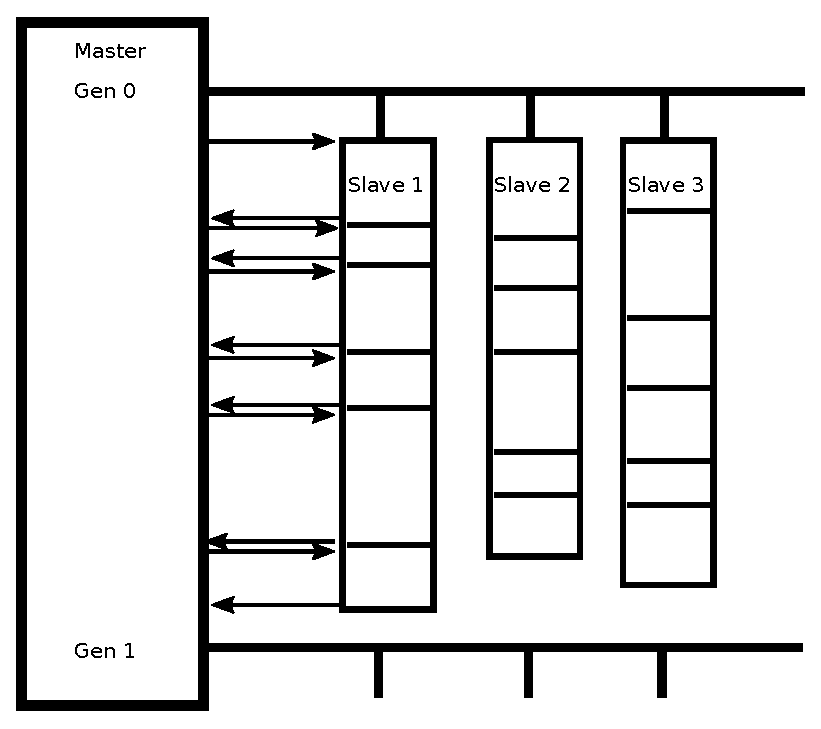
\includegraphics[angle=0,scale=0.65]{Master_slave.eps}
   \caption{Overview of parallel refinement process }
   \label{fevo-over}
\end{figure}

\begin{MacVerbatim}
   mpiexec -np 8 diffev -macro refinement.mac
\end{MacVerbatim}

the \Suite starts a master process that will in turn start np-1 slave 
processes. In each generation the master process will instruct the slaves
to perform several tasks. Lets say you you have a large population and
each individual simulation does not have to be repeated. The master will 
then instruct the slaves to start the calculation for the first np-1
members. As soon as a slave is finished, it will send back the result to 
the master and receive the instructions to start the calculations for
the next member. This communication is indicated by the arrows between the
 master and the first slave in Fig \ref{fevo-over}. In many cases the 
calculation times for each member will differ as indicated by the 
different vertical positions of the horizontal bars within each slave.
Ideally all slaves would terminate their last calculation at the same time. 
This would minimize idle time on the computer. This is, however,
difficult to enforce and some idle time for almost all slave can hardly be
avoided. 

If the computation time for all members is identical, the number of slaves
and the population size should be matched such that the population size is
an integer multiple of the number of slaves np-1. This will ensure that
all slaves will perform calculations for an identical number of members and
will be finished at the same time. If the population size is larger by
one member, a single slave will be busy with this last member while all
other slaves are just waiting for new instructions.

If the computation times for the different members differ but can be estimated 
ahead of times it is best to start to distribute the large jobs first and then
once these are done to hand out the shorter jobs. Those slaves that receive
the shorter jobs will perform calculations for more members that those 
slaves that receive the larger jobs. If the large jobs are handed out first, 
the chances are optimized that all the shorter jobs will finish roughly at the 
same time.

If the computation times cannot be estimated ahead of times, some idle time
is likely to occur. To reduce the amount of idle times each slave should perform
calculations for several members. As in the last paragraph, those slaves that
happen to receive larger jobs will perform calculations for fewer members. 
With several jobs per slave the fluctuations at the end should be about
half the computation time for an individual average job. 
If, as the other extreme, each slave were to 
calculate just one simulation, the one slave that takes the longest
calculation will force all other slaves to be idle until it is finished.
This will cause a huge amount of idle time.

At the moment the \Suite does not attempt to estimate how long
each calculation will take. There are just too many different parameters
that will influence the time like nanoparticle size, number of atoms, number
of atom types, time spend within a Monte-Carlo simulation etc. Given this
lack of information the idle time is minimized if each slave performs 
several calculations.  

The situation is slightly different if the calculations require the need 
to perform each simulation several times for a given member. This will be 
the case for example if you simulate small nanoparticles and the simulation
involves the creation of (randomly distributed) defects. As the individual
nanoparticle is small, its structure and as a consequence its powder 
diffraction pattern or PDF will not be a good representative of all possible 
structural conformations. You will have to repeat the simulation again for the 
same set of parameters. Afterwards all the individual powder pattern /PDF's
will have to be averaged. If an individual member has to be repeated N times,
the total number of simulations will of course be N times as large. To reduce 
the idle time the \Suite will hand out jobs for the first individual calculation
for each member first. Once all these are done the next individual calculations
will follow. All individual repetitions for an individual member likely
require a similar amount of time, while the requirements for different members 
may vary.

Once all members and all individual repetitions have been performed the \Suite
will have to average the temporary results. This averaging process can of 
course be performed in parallel as well. This raises two further issues 
related to the architecture of the computer at hand. 

A local computer or local compute server has an architecture similar to 
Fig. \ref{fevo-arch}. Several 
CPUs or cores perform the computing and MPI can distribute the workload onto 
these CPUs or cores. The CPUs share a common disk to store permanent data. 
At a large scale compute facility many of these units are combined. The local 
storage at each of these nodes often is a solid state memory instead of a 
traditional hard disk. A very large central disk provides storage space for 
global results. The scheduling process at such a high performance compute
center (HPC) typically give your job a privileged and sole access to all CPUs at 
a node and you process may request several nodes at the same time. The 
communication between the CPU's on a node and their local 
disk is fast, efficient and only interferes with you own jobs. The communication
to the central hard disk is common to all processes by all users at the HPC. 
Thus this communication should be reduced as much as possible as it may slow 
down your own process and that of other users as well. 

\begin{figure}
   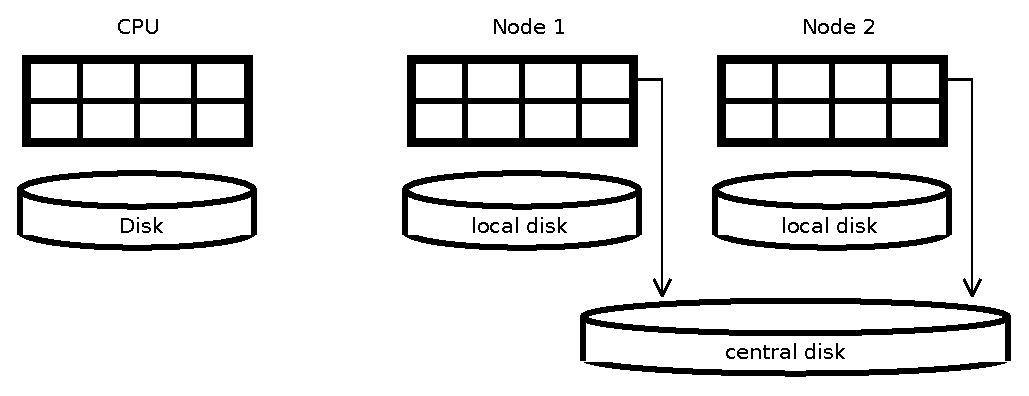
\includegraphics[angle=0,scale=0.65]{arch.eps}
   \caption{Simplified architecture of single PC with eight core CPU, left,
            and multi node HPC, right}
   \label{fevo-arch}
\end{figure}

The MPI distribution usually does not offer a direct assignment of a 
particular job to a specific core. This means, that the master process 
usually has no means to predict on which CPU a given calculation will occur. 

As of version 5.17.0 and later ones, the \Diffev section tries to optimize
the internal distribution of jobs onto the available nodes and their individual
cores as best as possible for any compute environment.

Keep in mind that we can have two different refinement situations:
\begin{itemize}
  \item The calculation for a member does not have to be repeated several 
        times
  \item The calculation for a member does have to be repeated several 
        times and the results need to be averaged once all calculations
        have been performed
\end{itemize}

Independent of this you may have two different compute architectures
available for your refinement:
\begin{itemize}
  \item A local PC or local small scale server with a single node
  \item A HPC center with many nodes, each node has its own local 
        storages common to all cores on this node
\end{itemize}

To match your refinement situation to the local architecture and to optimize
the performance \Diffev offers two different refinement styles:

\begin{MacVerbatim}
variable integer, nindiv
REF_NINDIV = 20
... diffev setup ...
pop_n[0] = 192
pop_c[0] = 192
... further diffev setup ...
... FIRST style
run_mpi discus, dis.diffev.mac, repeat:REF_NINDIV, compute:serial, logfile:/dev/null
...
... SECOND style
run_mpi discus, dis.diffev.mac, repeat:REF_NINDIV, compute:parallel, logfile:/dev/null
run_mpi kuplot, kup.diffev.mac, repeat:REF_NINDIV, compute:serial, logfile:/dev/null
\end{MacVerbatim}

Within the first style \Diffev will start pop\_c calculations. here in this
example arbitrarily set to 192. These 192 calculations will be distributed in
parallel onto the available CPUs. If the model requires any repetitions, the
\Discus macro here {\tt dis.diffev.mac} will have to include a loop over these
repetitions. The \Discus macro also needs to include a {\tt branch} to the 
\Kuplot section to calculate the R-value. As all repetitions for a given member 
are performed serially on a single CPU, you can write the \Discus output
data either onto a hard disk or directly into the \Kuplot memory space. The 
latter is done by prepending the output file name by the string {\tt kuplot}.
See the \Discus manual for further details. As the individual calculations 
during the refinement are temporary data of no long term relevance, it is a
good idea to avoid disk input/output. Thus the internal write is recommended.

Within the second style \Diffev will start pop\_c times nindiv calculations.
In this example this results in a total of 3840 calculations that can all be
performed in parallel. Each time the \Discus macro {\tt dis.diffev.mac} will
calculate data for just one member and will have to write these data onto a 
disk. Once all 3820 calculations are finished, \Diffev will instruct \Kuplot 
in a second parallel job to average all calculations for a given member and to 
calculate the corresponding R-value. As a single \Kuplot slave needs to average 
all repetitions, the parameter {\tt "compute"} is set to {\tt "serial"}. 
In this second model you need to write 
the data onto a disk, as the memory requirements would be too large for 
internal storage. A more stringent reason to write the data onto disk is that 
a single slave will perform calculations for members and individual repetions
in an unpredictable sequence. One can expect that the calculations for one 
member are performed by different slaves.

Now lets have a look at strategies to run these two different schemes on the 
two compute architectures. Common to both architectures, you will have np-1
processors available to perform actual calculations while the one master
processor keeps itself busy with administrative tasks. All slave processors 
should perform several jobs as this minimizes the risk of a long idle time 
at the end of a generation. 

\begin{itemize}
  \item Single PC or small server \newline
        On these systems several users might be active or you may run several 
        refinements or other tasks. As these tasks can take up idle time the
        following rules can be relaxed.
      \begin{itemize}
          \item No individual repetitions. The number of members should be
                an integer multiple of (np-1). To reduce the idle time the
                multiple should be high. 
          \item With repetitions. Both computation models are an option. If
                the calculation times are long per repetition you will not
                do too many disk I/Os to slow you down or to risk the integrity
                of your hardware. If the calculation time is fairly short, it
                might be kinder to your hardware to choose th first computational 
                model as temporary data can (and should) be saved internally.
      \end{itemize}
   \item High Performance Compute center \newline
         On these systems you will have sole access to a given node and its CPU.
         Local disk I/O is fast and does not cause wear and tear if the storage
         is a solid state disk. As you are the sole user, idle time should be
         minimized. A lot of disk I/O across the network onto the central disk
         will be frowned upon and should be reduced as much as possible.
      \begin{itemize}
          \item No individual repetitions. The number of members should be
                an integer multiple of (np-1). To reduce the idle time the
                multiple should be high. As a single node often has 24 or more
                CPUs request few nodes and long wall time instead.
          \item With repetitions. Both computation models are an option. The 
                second model makes better use of the many processors available.
                As of version 5.17.0 \Diffev will place all individual repetitions
                for one member onto the same node. If the local storage at a node 
                is a solid state disk the temporary storage will not significantly 
                slow down your process. Thus different slave processes that run on 
                the same node can calculate individual repetitions for any of the
                members on that node. The number of members should still be 
                an integer multiple of (np-1) but the factor can be reduced. The
                (large) number of individual repetitions will level out the workload
                at each core of a given node.
      \end{itemize}
\end{itemize}
%------------------------------------------------------------------------
